\section{Modelo de Comportamiento}
\label{sec:behaviorModel}

El modelo de comportamiento se centra en los \textbf{flujos que cruzan varias capas de la aplicación} y que, por tanto, son especialmente relevantes para verificar la coherencia entre interfaz, autenticación, servicios de dominio y persistencia. Para ello se emplean diagramas de secuencia y de estados de \textit{UML}, adecuados para representar interacciones entre componentes y evolución de objetos dentro del sistema \citep[Ch.~5]{sommerville}.

\subsection{Criterio de selección de escenarios}

El sistema contiene numerosos flujos de consulta, alta, edición y administración. Sin embargo, modelarlos todos mediante diagramas de comportamiento produciría documentación redundante respecto al modelo de casos de uso y al modelo conceptual. Por este motivo, se seleccionan los escenarios que concentran mayor riesgo funcional o que conectan varias partes de la aplicación:

\begin{itemize}
    \item \textbf{Acceso y protección de rutas}: representa el flujo transversal de autenticación, autorización y control de sesión que condiciona el uso del resto de módulos.
    \item \textbf{Pedido, reparto y validación mediante \textit{QR}}: recoge el flujo principal de \texttt{M4}, donde intervienen interfaz, \textit{API}, servicios de dominio, persistencia, visita comercial y confirmación de entrega.
    \item \textbf{Ciclo de estados de pedido, reparto y cobro}: resume la evolución permitida de las entidades operativas más sensibles, evitando estados incoherentes entre pedido, entrega y seguimiento económico.
\end{itemize}

Las funcionalidades adicionales de \texttt{M8} no se modelan en este apartado porque forman parte de trabajo futuro y no del comportamiento operativo principal de la aplicación.

\subsection{Diagramas de secuencia}

Los diagramas de secuencia muestran cómo colaboran los elementos principales del sistema en dos recorridos representativos: el acceso protegido y la operativa de pedido con reparto. Ambos casos permiten observar el paso desde la interacción del usuario hasta la validación de reglas, consulta o modificación de datos y devolución de respuesta a la interfaz.

La Figura~\ref{fig:seq-login-protected-access} resume el \textbf{acceso al sistema}: el usuario introduce credenciales, \texttt{Auth.js} \citep{authjsdocs2026} valida la identidad contra \texttt{PostgreSQL} \citep{postgresdocs2026}, se genera una \textbf{\textit{cookie} de sesión segura} y la capa de \textbf{protección de rutas} controla el acceso posterior a zonas privadas.

\begin{figure}[p]
    \centering
    \rotatebox{90}{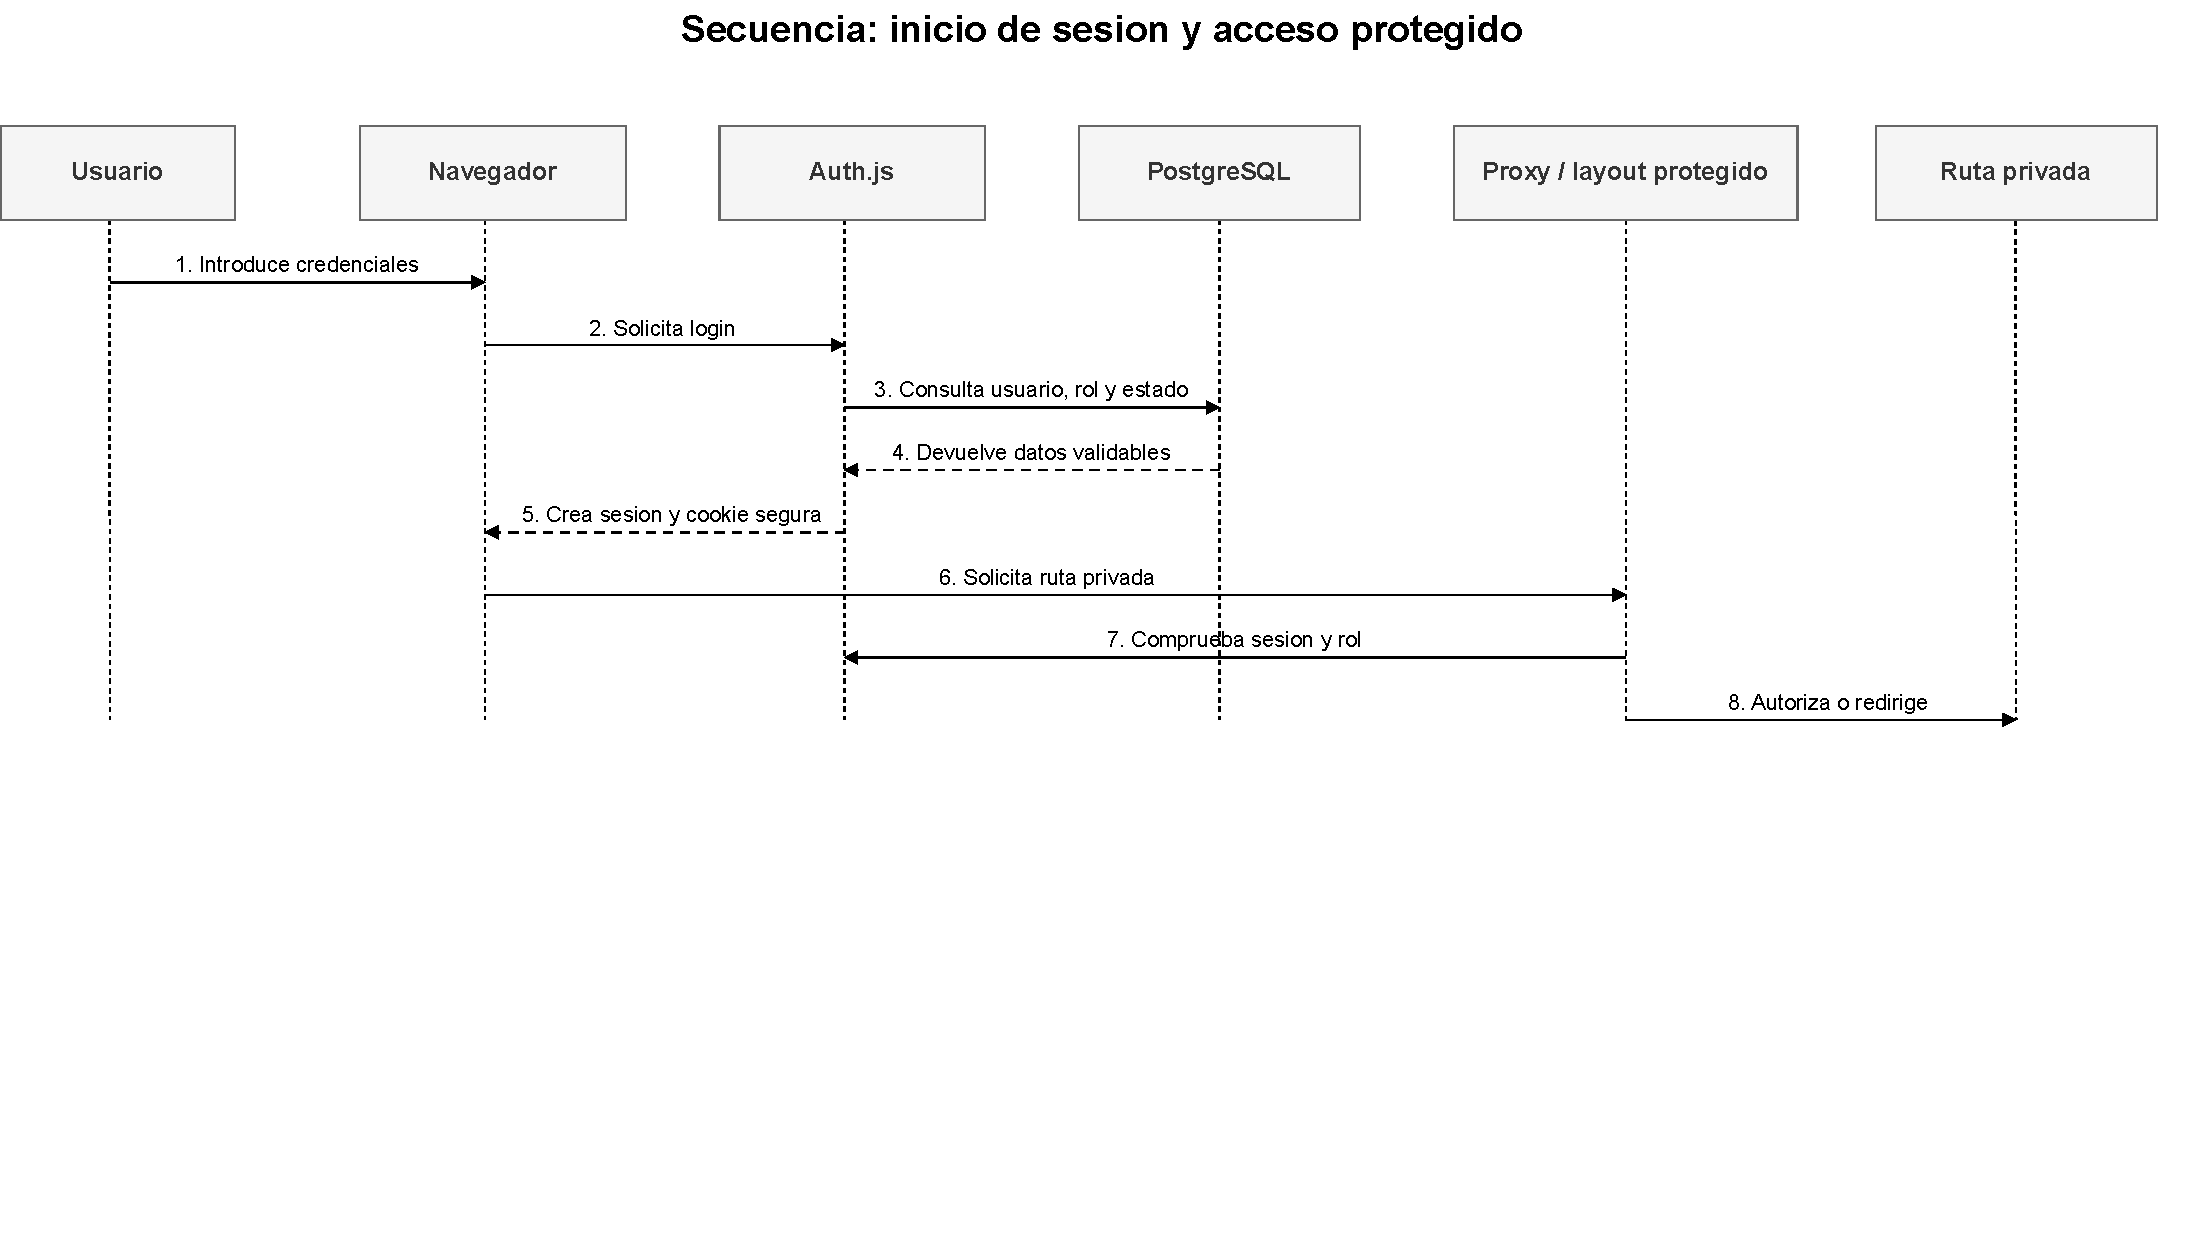
\includegraphics[width=0.88\textheight,height=0.98\textwidth,keepaspectratio]{./figures/UML/MCO/sequence-login-protected-access.pdf}}
    \caption{Diagrama de secuencia: inicio de sesión y acceso protegido}
    \label{fig:seq-login-protected-access}
\end{figure}

La Figura~\ref{fig:seq-order-qr-delivery} recoge el \textbf{flujo de pedido y reparto}: la pantalla de pedidos registra líneas, la \textit{API} valida productos y tonos, el servicio de dominio persiste el pedido, se vincula la entrega a una visita comercial y el \textit{QR} permite confirmar la entrega desde el detalle operativo.

\begin{figure}[p]
    \centering
    \rotatebox{90}{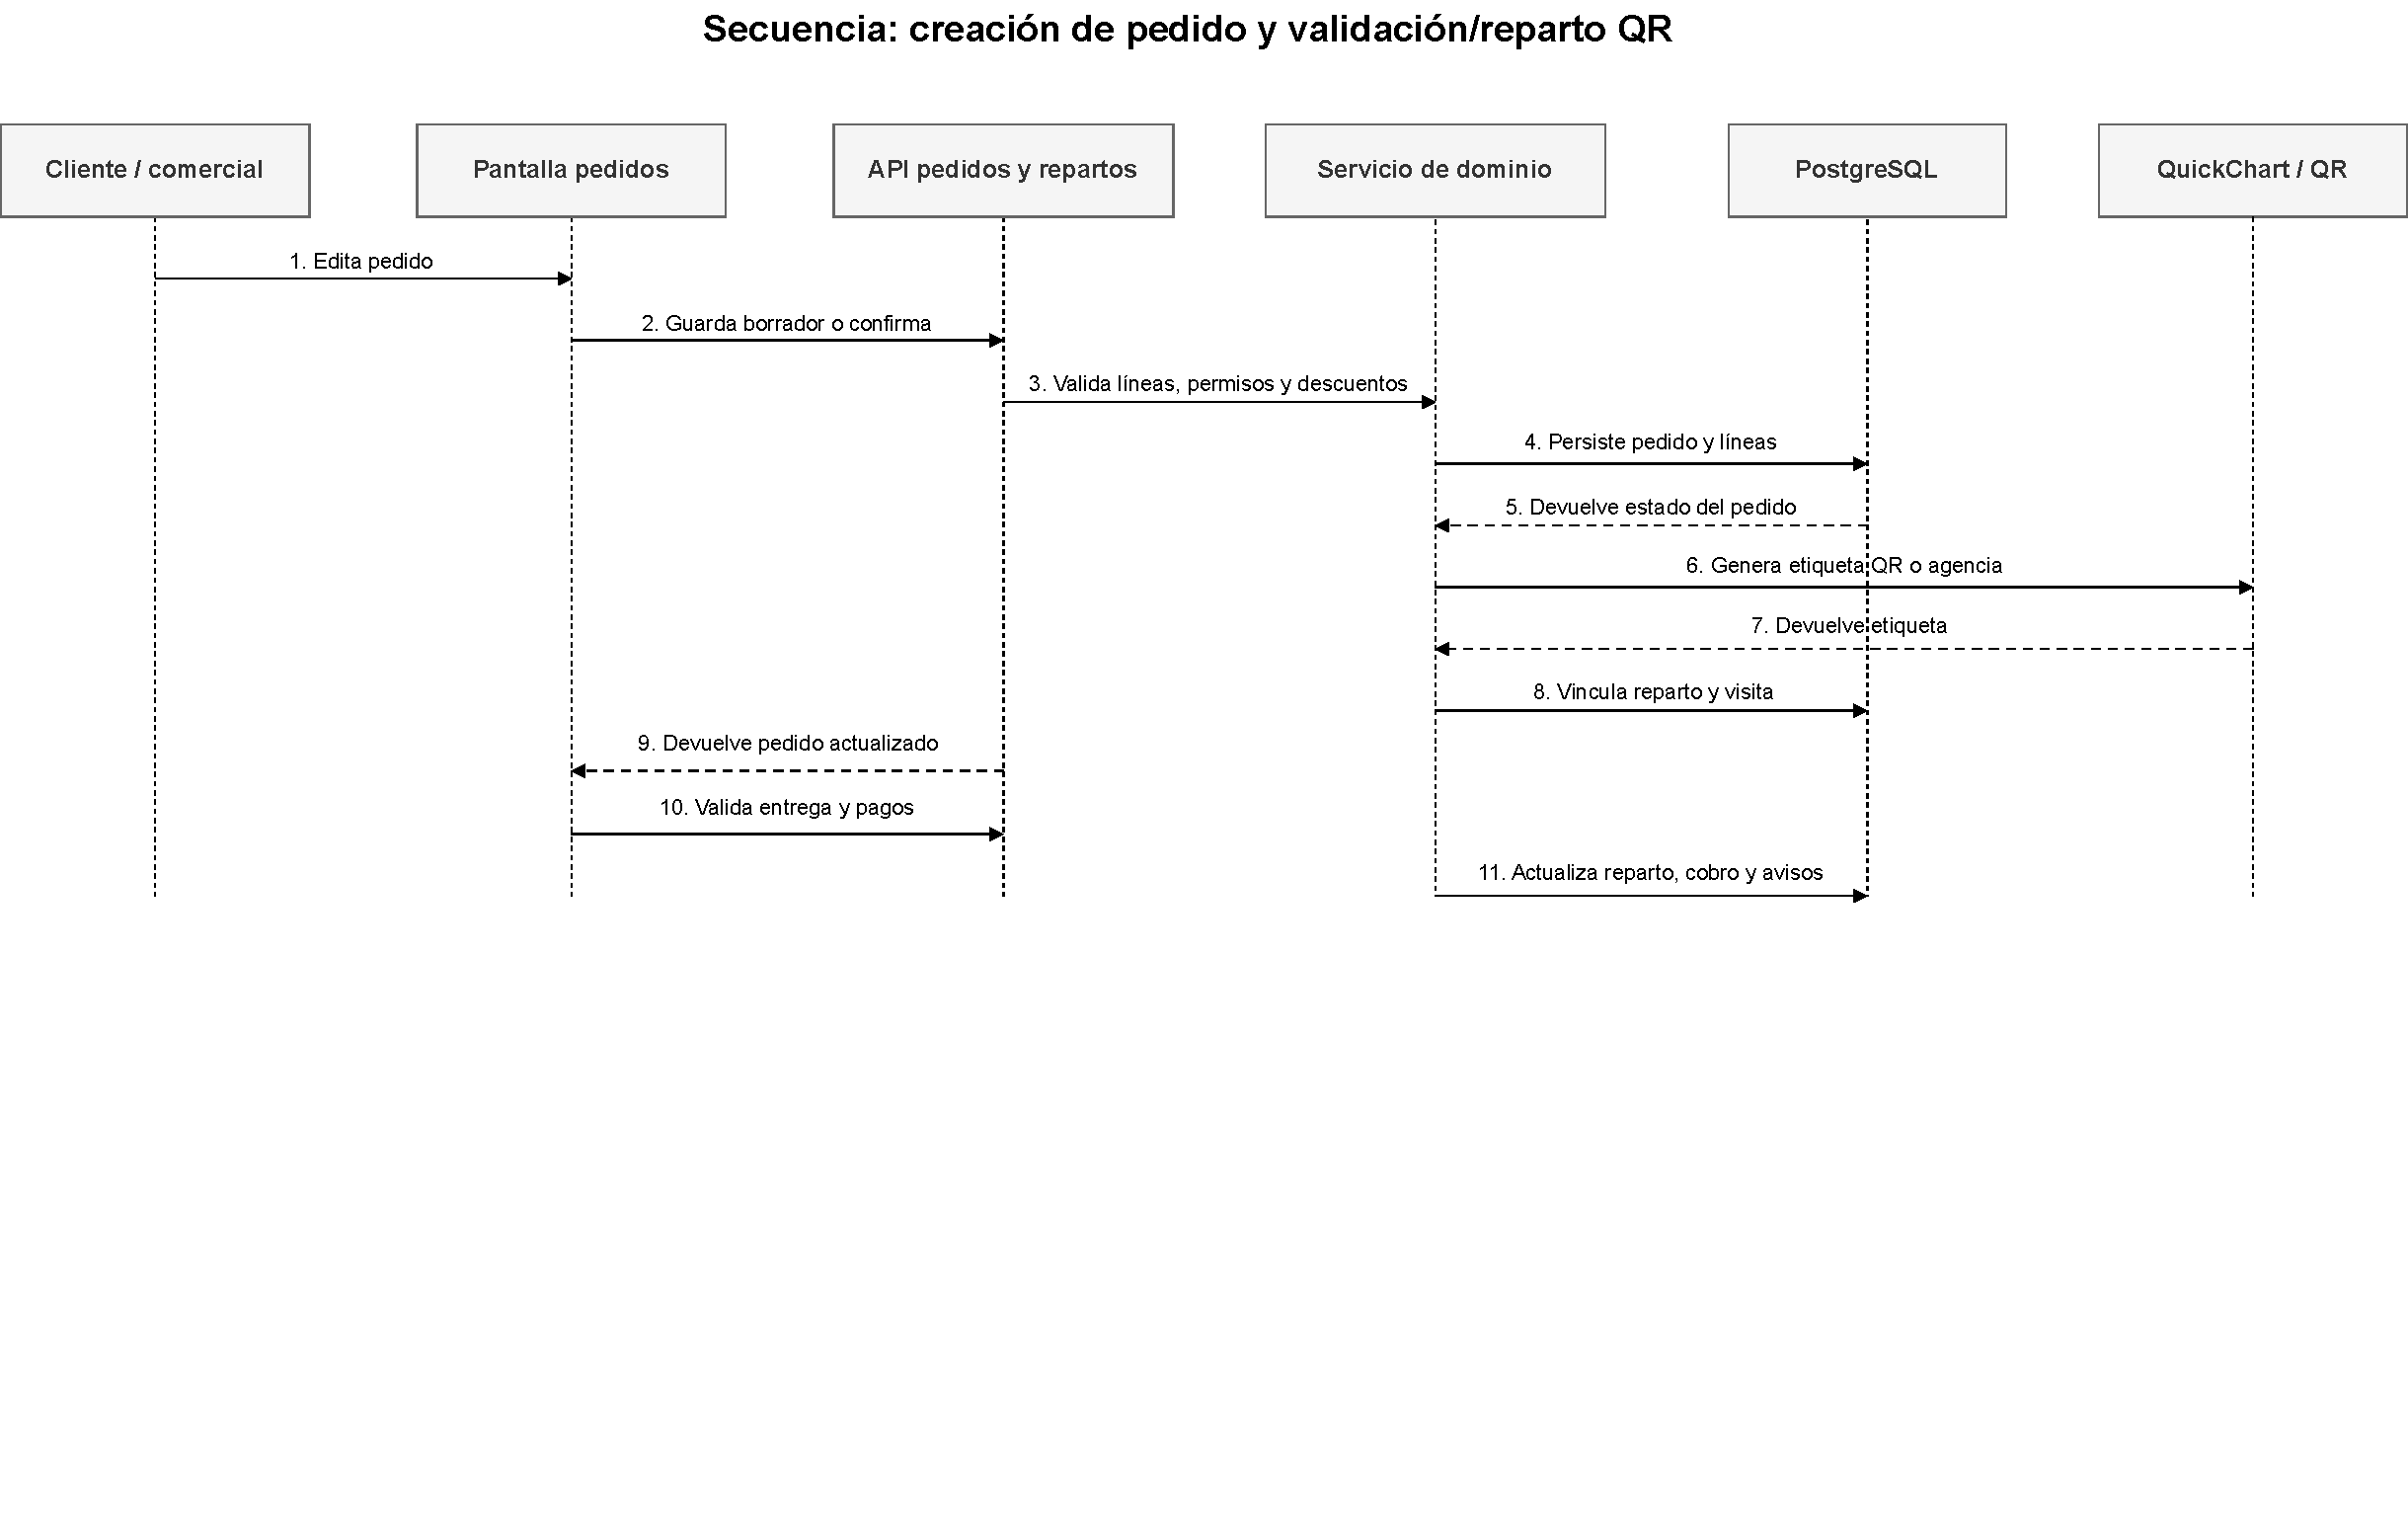
\includegraphics[width=0.88\textheight,height=0.98\textwidth,keepaspectratio]{./figures/UML/MCO/sequence-order-qr-delivery.pdf}}
    \caption{Diagrama de secuencia: creación de pedido y validación/reparto QR}
    \label{fig:seq-order-qr-delivery}
\end{figure}

\subsection{Diagrama de estados del ciclo de pedido, reparto y cobro}

El flujo de \texttt{M4} combina tres ciclos relacionados: el \textbf{estado comercial del pedido}, el \textbf{estado logístico del reparto} y el \textbf{estado de cobro}. La Figura~\ref{fig:state-order-delivery-payment} representa estos estados de forma conjunta para mostrar que la entrega y el cobro no evolucionan de manera aislada, sino condicionadas por las reglas de negocio del pedido.

\begin{figure}[p]
    \centering
    \rotatebox{90}{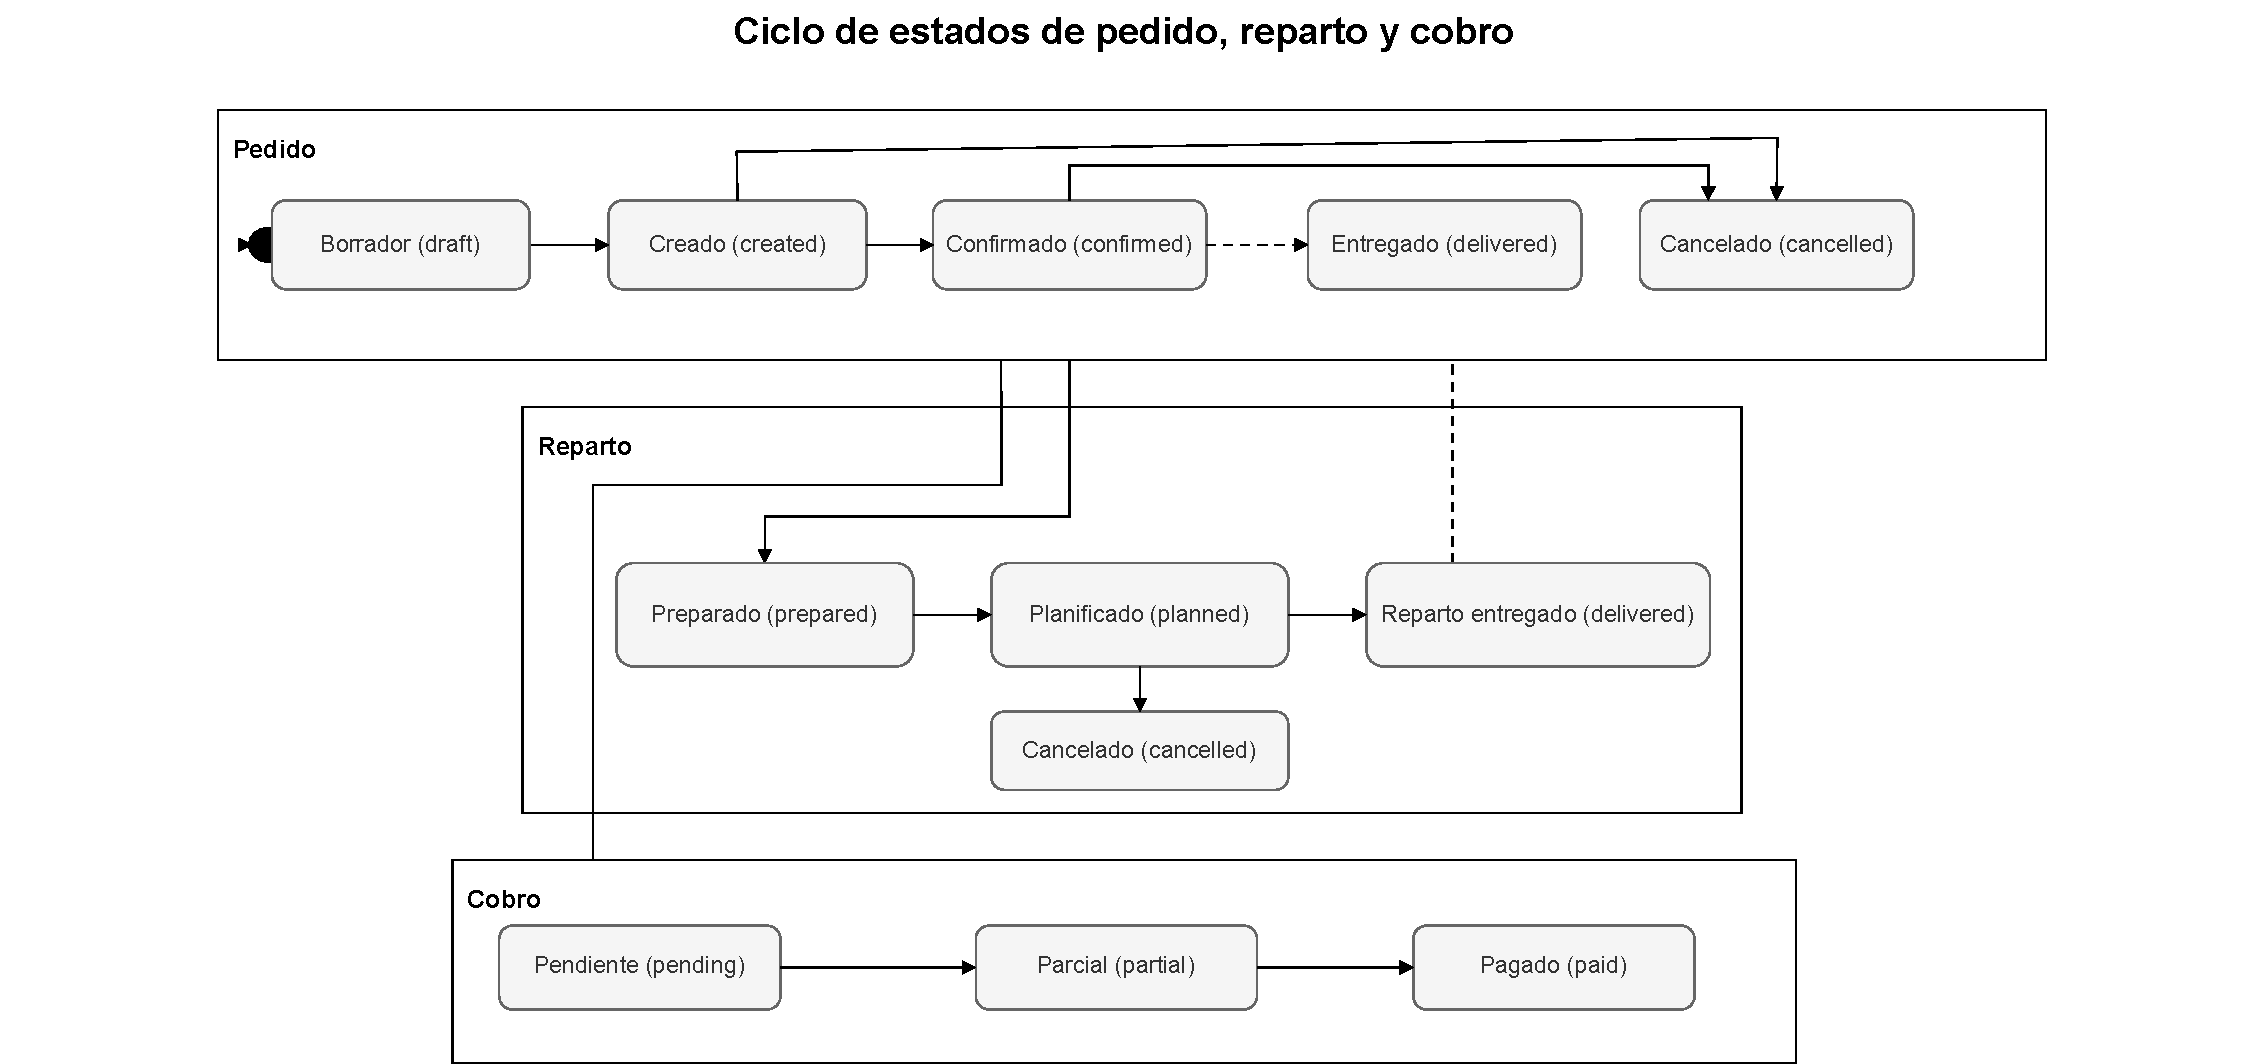
\includegraphics[width=0.88\textheight,height=0.98\textwidth,keepaspectratio]{./figures/UML/MCO/order-delivery-payment-state.pdf}}
    \caption{Diagrama de estados: ciclo de pedido, reparto y cobro}
    \label{fig:state-order-delivery-payment}
\end{figure}

En el \textbf{pedido}, el sistema distingue un borrador interno \texttt{draft}, un pedido registrado como \texttt{created}, la confirmación \texttt{confirmed}, la entrega completa \texttt{delivered} y la cancelación \texttt{cancelled}. El \textbf{reparto} se prepara sobre pedidos confirmados, puede quedar \texttt{prepared}, planificarse como \texttt{planned} cuando se vincula a una visita comercial, marcarse como \texttt{delivered} tras la validación o cancelarse si la operación deja de ser válida. Por último, el \textbf{cobro} permanece \texttt{pending} mientras exista saldo pendiente y pasa a \texttt{paid} cuando los pagos registrados cubren el importe total del pedido.
